\documentclass[a4paper]{article}

%% Language and font encodings
\usepackage[english]{babel}
\usepackage[utf8x]{inputenc}
\usepackage[T1]{fontenc}

%% Sets page size and margins
\usepackage[a4paper,top=3cm,bottom=2cm,left=3cm,right=3cm,marginparwidth=1.75cm]{geometry}
\usepackage[section]{placeins}
%% Useful packages
\usepackage{amsmath}
\usepackage{graphicx}
\usepackage[colorinlistoftodos]{todonotes}
\usepackage[colorlinks=true, allcolors=blue]{hyperref}

\title{Chapter 8 Autocorrelation Assignment}
\author{Petra Guy}

\begin{document}
\maketitle

\section{Introduction}
I wrote three scripts (so far!). Initially I wrote a python-ish functions script, 
but I wanted to make this run using Rscript, which I couldnt.
 I therefore rewrote I long ugly code, thinking that if I ran that
  from Rscript it would simple run through line by line. But the 
  load command would not work. I also checked the results of my 
  calculations against the R acf() function, and they were the same, 
  so I wrote another script using that. 

\section{Graphs}

\begin{figure}

\centering
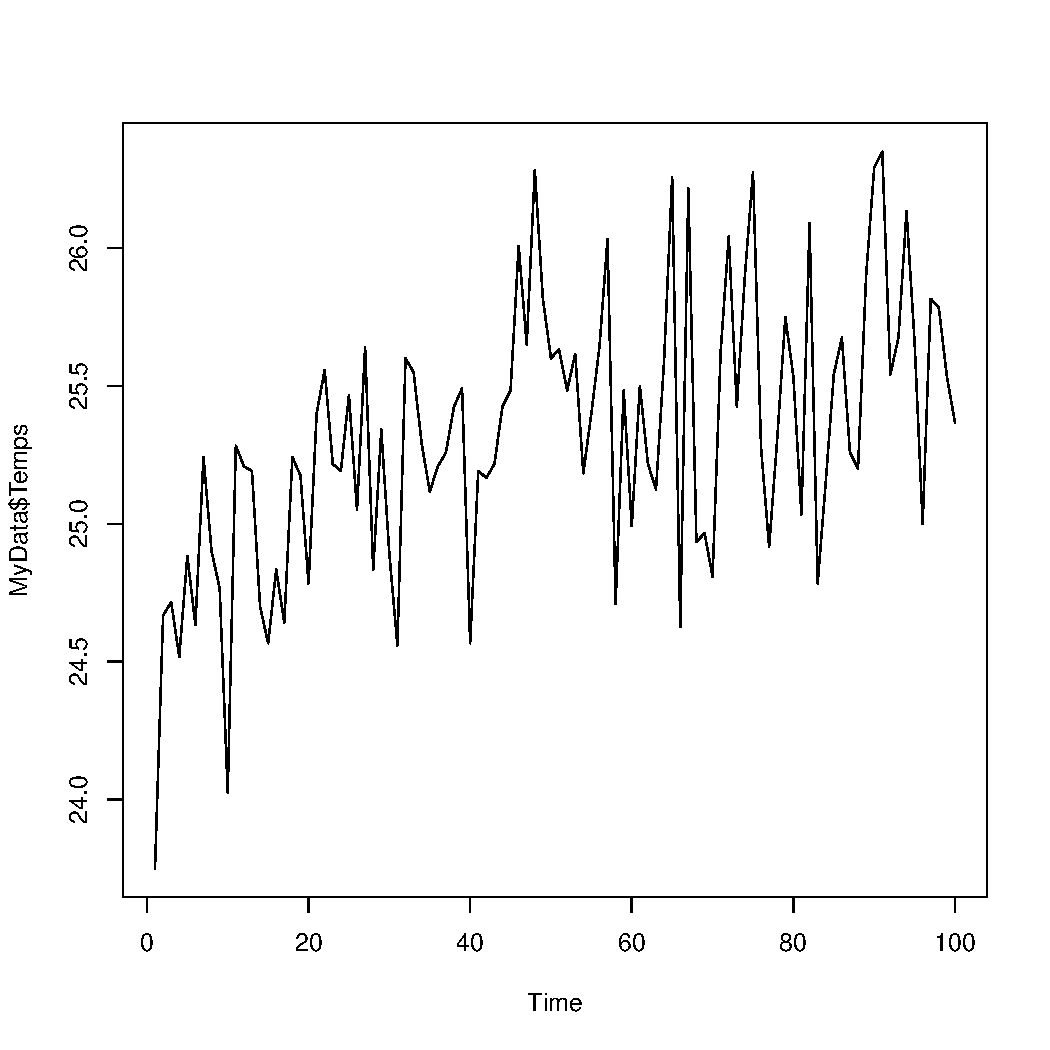
\includegraphics[width=0.5\textwidth]{TAutocorrtimeseries1.pdf}
\caption{\label{fig:TAutocorrtimeseries1.pdf}Time series plot.}

\centering
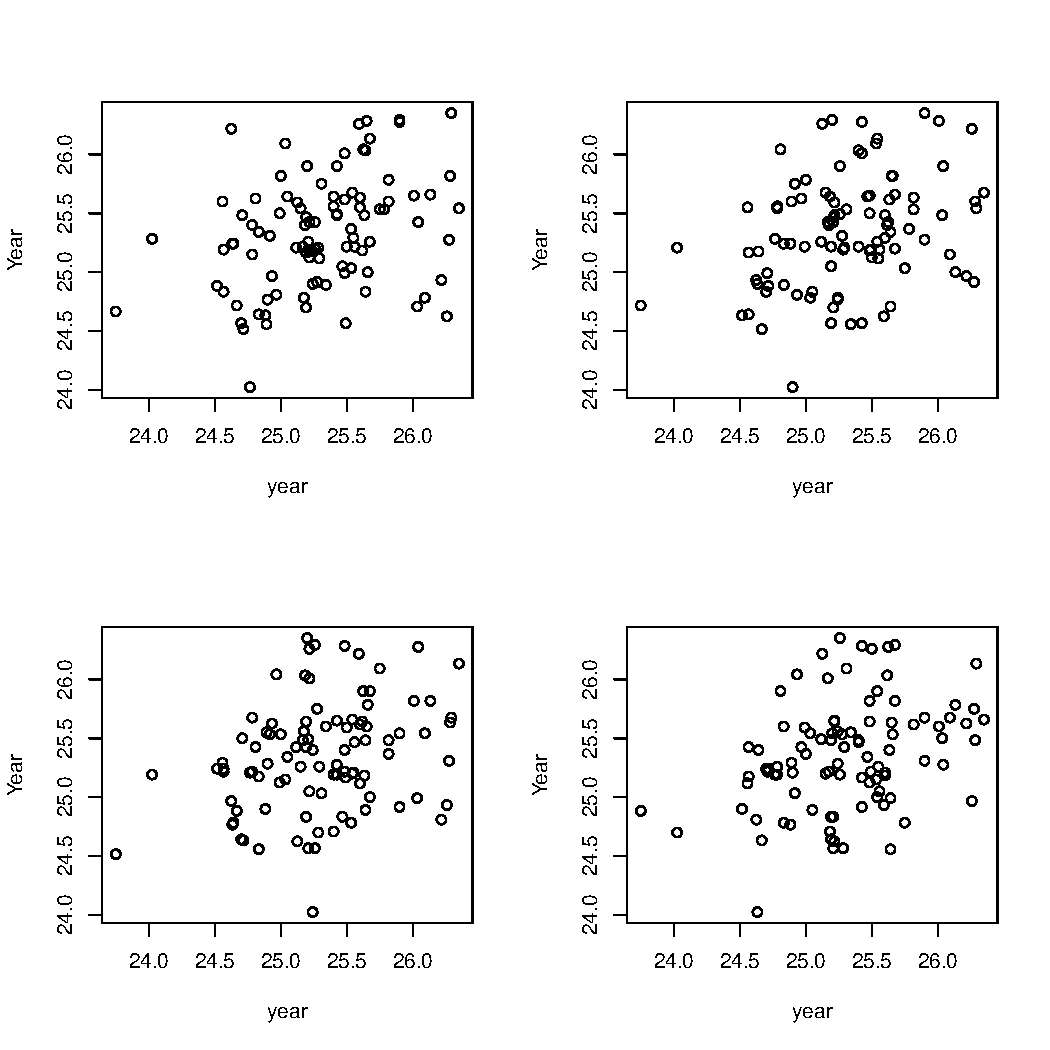
\includegraphics[width=0.5\textwidth]{TAutocorrtimeseries2.pdf}
\caption{\label{fig:TAutocorrtimeseries2.pdf}Scatter plots of years for lags of 1 to 4 years.}

\centering
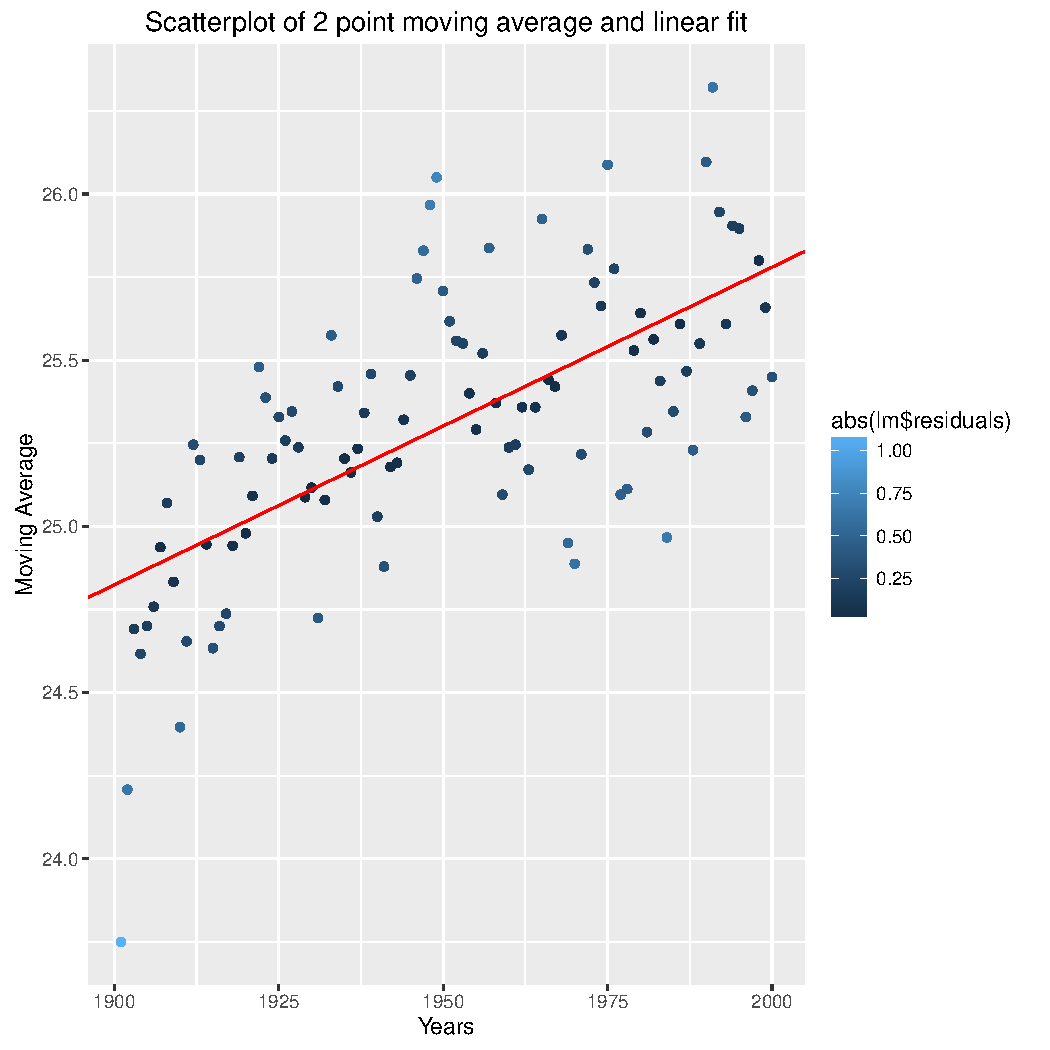
\includegraphics[width=0.5\textwidth]{TAutocorrmovingavg.pdf}
\caption{\label{fig:TAutocorrmovingavg.pdf}Plot of moving averages and fit.}
\end{figure}



\clearpage
\newpage
\mbox{~}
\clearpage
\newpage
\end{document}



